\documentclass[11pt]{article}
\renewcommand{\baselinestretch}{1.20} 
\usepackage[utf8]{inputenc}
\usepackage[english]{babel}
\usepackage{graphicx}
\usepackage{wrapfig}
\usepackage{subcaption}
\usepackage{enumitem}
\usepackage{geometry}
\usepackage{xcolor}
\usepackage{float}
\usepackage{mdframed}
\usepackage{fancyhdr}
\usepackage{lastpage}
\usepackage{listings}
\usepackage{booktabs}
\definecolor{codegray}{gray}{0.9}
\newcommand{\code}[1]{\colorbox{codegray}{\texttt{#1}}}
\newcommand{\tabitem}{~~\llap{\textbullet}~~}
\geometry{a4paper, total={170mm,237mm}, left=20mm, top=20mm}
\setlength{\abovecaptionskip}{15pt plus 3pt minus 2pt}

\pagestyle{fancy}
\fancyhf{}
\rfoot{Side \thepage \hspace{1pt} / \pageref{LastPage}}
\begin{document}
    
    % Title page
    \begin{titlepage}
    \centering
	
\includegraphics[width=0.35\textwidth]{Projectdoc/Assets/Illustrationer/aau_logo_en.pdf}\par\vspace{1cm}
	{\scshape\Large Struktureret System Udvikling\par}
	\vspace{0.2cm}
	{\huge\bfseries Workshop 3\par}
	\vspace{0.2cm}
	{\scshape\Large ITC - B125\par}
	\vspace{2cm}
	{\Large\itshape 
    	Mikkel Steen Hansen\\
        Benjamin Bach Jensen\\
        Daniel Vestergaard Jensen\\
    \par}
	\vfill
	\vfill
\end{titlepage}
    
    % Table of contents
    \renewcommand{\baselinestretch}{0.8}
    \tableofcontents
    \renewcommand{\baselinestretch}{1.20}
    \newpage
    
    \section{Beskrivelse}
    \textbf{Mini projekt: ruter station}\\
    \noindent
    Dagens workshop omhandler testing og fejlbehandling.\\
    Tanken bag projektet er at gruppen har fået to funktioner \textit{SquareRoot} og \textit{BubbleSort}, der nu videre skal anvendes i sammenhæng til at sortere en gruppering af tal og finde:
    \begin{itemize}
        \item Et gennemsnit.
        \item De tre mindste tal.
        \item De tre største tal.
        \item Det mest afvigende fra gennemsnittet.
        \item Det mindst afvigende fra gennemsnittet.
    \end{itemize}
    \noindent
    Disse to førnævnte funktioner er dog ikke fuldt funktionelle da de ikke returnerer de forventede resultater.
    Denne konklusion kan uddrages fra udførelsen af en Blackbox test. Blackbox testen kigger kun på input og output. Den kan validere programmet ved at sammenholde forventet output med det egentlige output, baseret på det givne input.
    \newpage
    \section{Blackbox testing}
    \subsection{SquareRoot}
    For \textit{SquareRoot} har gruppen dannet følgende skema for mulige inputs, samt hvad disse returnerede under første gennemgang (inden kode rettelse), og hvad der faktisk forventes som resultat.
    \begin{center}
        \begin{tabular}{ |c|c|c| }
            \hline
             Testet input & Forventet resultat & Faktisk resultat \\
            \hline
             Bogstaver & - & - \\
              A & Ugyldigt & Loop med 0 som resultat\\
              V & Ugyldigt & Loop med 0 som resultat \\
              Å & Ugyldigt & Loop med 0 som resultat \\
              * & Ugyldigt & Loop med 0 som resultat \\
             Hele tal \textless 0 & - & - \\ 
              -2869 & Ugyldigt & Loop med 686467 som resultat,\\ 
              && før segmenteringsfejl\\
              -4 & Ugyldigt & Loop med 1.33438 som resultat,\\ 
              && før segmenteringsfejl \\
             Decimal tal \textless 0 & - & -\\
              -954.459 & Ugyldigt & Loop med 75902.4 som resultat,\\ 
              && før segmenteringsfejl\\
              -8.5 & Ugyldigt & Loop med 5.337551 som resultat,\\ 
              && før segmenteringsfejl \\
             Tallet 0 & 0 & 0 \\
             Hele tal \textgreater 0 & - & - \\
              5625 & 75 & Loop med 2.63878e+006 som resultat,\\ 
              && før segmenteringsfejl \\
              2869 & 53.5630469 & Loop med 686467 som resultat,\\ 
              && før segmenteringsfejl \\
              15 & 3.8729833 & Loop med 18.7647 som resultat,\\ 
              && før segmenteringsfejl \\
              4 & 2 & Loop med 1.33438 som resultat,\\ 
              && før segmenteringsfejl \\
             Decimal tal \textgreater 0 & - & - \\
              5625.5625 & 75.0037499 & Loop med 2.63878e+006 som resultat,\\ 
              && før segmenteringsfejl \\
              2869.9682 & 53.5720841 & Loop med 686467 som resultat,\\ 
              && før segmenteringsfejl \\
              15.51 & 3.9382737 & Loop med 18.7647 som resultat,\\ 
              && før segmenteringsfejl \\
              4.0 & 2.0 & Loop med 1.33438 som resultat,\\ 
              && før segmenteringsfejl \\
             \hline
        \end{tabular}
    \end{center}
    
    \newpage 
    \subsection{BubbleSort}\noindent
    For \textit{BubbleSort} har gruppen dannet følgende skema for mulige inputs, samt hvad disse returnerede under første gennemgang (inden kode rettelse), og hvad der forventes som resultat.
    \begin{center}
        \begin{tabular}{ |c|c|c| } 
            \hline
             Testet input & Forventet resultat & Faktisk resultat \\
            \hline
             Bogstaver & - & - \\
              CBDAFEHIG & ABCDEFGHI eller & \\ 
              &65 66 67 68 69 70 71 72 73 & 67 \\
              VXURWTSZY & RSTUVWZXY eller & \\ 
              & 82 83 84 85 86 87 88 89 90 & 88 \\
              ÄÅØÆëæøïå & åëïÄÅæÆøØ eller & \\ 
              & 134 137 139 142 143 145 146 155 157 & -59 \\
              +\$-!/*\#\&= & !\#\$\&*+-/= or & \\
              & 33 35 36 38 42 43 45 47 61 & 43 \\
             Hele tal \textless 0 & - & - \\
              -1500 -2679 -1890 -1233 -1967 & -1233 -1456 -1500 -1785-1967 & \\
              -2255 -1456 -1785 -2122 & -1890 -2122 -2255 -2679 & -1500\\ 
              &&\\
              -4 -2 -5 -1 -3 -9 -6 -7 -8 & -1 -2 -3 -4 -5 -6 -7 -8 -9 & -2\\ 
             Decimal tal \textless 0 & - & -\\
              -954.459 -199.991 -956.569 -2856.2750 & -199.991 -325.895 -457.835 -954.459 & \\
              -2111.1112 -2574.3567 -325.895 -457.835 & -956.569 -1046.4785 -2111.1112 -2574.3567 & \\ 
              -1046.4785 & -2856.2750 & -199 \\ 
              &&\\
              -8.5 -4.6 -2.8 -1.1 -3.2 -9.2 -6.7 -5.3 -7.4 & -1.1 -2.8 -3.2 -4.6 -5.3 -6.7 -7.4 -8.5 -9.2 & -4\\ 
             Hele tal \textgreater 0 & - & - \\
              1500 2679 1890 1233 3657 & 1111 1233 1500 1890 2679 & \\ 
              4782 3589 9999 1111 & 3589 3657 4782 9999 & 2679\\
              &&\\
              4 2 5 1 9 7 6 8 3 & 1 2 3 4 5 6 7 8 9 & 4 \\
             Decimal tal \textgreater 0 & - & - \\
              954.459 199.991 956.569 2856.2750 & 199.991 357.428 564.249 894.352 & \\ 
              9999.1111 1111.9999 564.249 357.428 & 954.459 956.569 1111.9999 2856.2750 & \\ 
              894.352 & 9999.1111 & 954\\ 
              &&\\
              8.5 4.6 2.8 1.1 9.3 3.2 7.9 5.6 6.3 & 1.1 2.8 3.2 4.6 5.6 6.3 7.9 8.5 9.3 & 8\\ 
             Blandede Tal & - & -\\
              1 -4 5.8 -7.2 9 -9 1.5 -1 6 & -9 -7.2 -4 -1 1 1.5 5.8 6 9 & 1 \\
              2 -1  569 -204 999 -111 5 -4 0 & -204 -111 -4 -1 0 2 5 569 999 & 2\\
             \hline
        \end{tabular}
    \end{center}
    
    \newpage \noindent
    Efter disse overstående resultater har gruppen foretaget rettelser af disse to funktioner ved anvendelse af Whitebox testing. Denne fejlfindings metode består i en gennemgang, først i en flowgraf ved dens forventede resultat, for forudbestemte muligheder eller inputs, og dernæst også ved nærmere inspektion af selve koden, samt dens faktiske resultater.
    
    \section{Whitebox testing}
    \subsection{SquareRoot}
    \noindent
    For \textit{SquareRoot} har gruppen dannet følgende flowgraf:\\
    \begin{table}[H]
        \begin{minipage}{.7\textwidth}
            \begin{figure}[H]
                \centering
                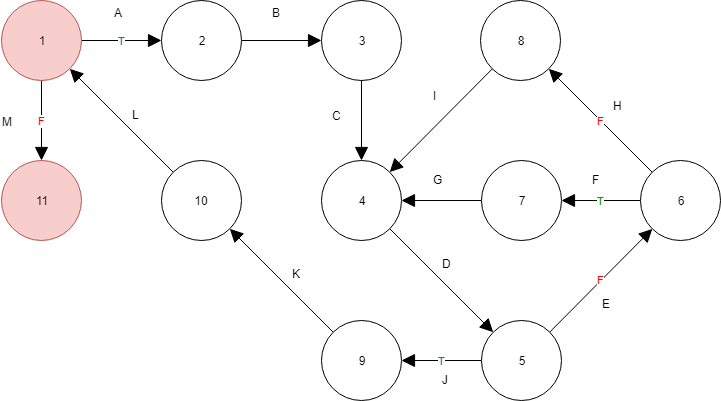
\includegraphics[width=1\textwidth,angle=0]{Struktureret_System_Udvikling/Workshop_3/SquareRoot_FlowGraph.png}
                \caption{SquareRoot FlowGraph Diagram}
                \label{fig:SquearRootGraph}
            \end{figure}
        \end{minipage}
        \begin{minipage}{.3\textwidth}
            \quad
            \begin{tabular}{lllll}
                1 & Main While loop\\
                2 & Get number input\\
                3 & SquareRoot\\
                4 & Sqrt\\
                5 & Is result found?\\
                6 & Is the guess too high?\\
                7 & Guess is too high\\
                8 & Guess is too low\\
                9 & Result found \\
                10 & Print result\\
                11 & End the program\\
            \end{tabular}
        \end{minipage}
    \end{table}
    \noindent
    Og kan derfor, ved en program kørsel forvente en gennemgang i ruterne:\\
    \textit{A-B-C-\{D-E-[F-G/H-I]\}*"Nødvendige gæt"-D-J-K-L-M}\\
    Hvor \{ - \} definerer et loop af en vis størrelse, der altid skal opfylde det beskrevne mønster.\\
    Den eneste undvigelse kan ses ved \textit{F-G} der også kan være beskrevet ved ruten \textit{H-I}.\\
    \\
    Efter første gennemgang kan det konkluderes at funktionen tager følgende rute:\\
    \textit{A-B-C-D-E-F-G-D-E-F-G-D-E-F-G-....} Dette tyder på at funktionen går i loop ved funktionen \textit{sqrt} under check på gættets størrelse i forhold til det indsatte tal, og herefter udskriver "Too High".
    Ved nærmere inspektion kan det også fra gennemgangens resultat, ses at det reelt indtastet tal, som er 4 i denne test, nu er blevet til 16. En kombination af disse betyder, at tallet kun vil blive mindre, da gættet er klassificeret som værende "Too High", og derved aldrig rammer det originale tal, der desuden også er blevet kvadreret.
    \begin{figure}[H]
        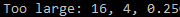
\includegraphics[width=0.3\textwidth,angle=0]{Struktureret_System_Udvikling/Workshop_3/Udklip.PNG}
        \label{fig:Udklip}
    \end{figure}
    \noindent
    Disse fejl kan rettes i funktionen SquareRoot1, hvor \code{res = sqrt(val * val, val / 2.0, 0.5);} skal rettes til \code{res = sqrt(val, val / 2.0, 0.5);} og i funktionen sqrt, hvor \code{if (tal + EPS \textgreater tmp)} skal rettes til \code{if (tal + EPS \textless tmp)}.
    Efter næste gennemgang kan det dog stadig ses, at funktionen ikke tager den forventede rute, da ruten stadig er det samme loop, for det efterspurgte tal (i dette tilfælde 16). Dog kan der denne gang også ses ud fra gennemgangens resultatet af det tredje tal "Step", hvilket bliver anvendt til at beregne næste gæt, bliver mindre og mindre.
    \begin{figure}[H]
        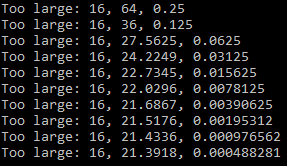
\includegraphics[width=0.3\textwidth,angle=0]{Struktureret_System_Udvikling/Workshop_3/Udklip2.PNG}
        \label{fig:Udklip2}
    \end{figure}
    \noindent
    Også ved at give funktionen et andet input, og derved gennemgå ruten \textit{...D-E-H-I} i stedet for \textit{...-D-E-F-G}, vil funktionen give det forventede resultat.
    Efter en videre inspektion af forskellen på disse, kan der konkluderes at fejlen ligger i funktionen \textit{sqrt}, i tjekket for om gættet er for høj, hvor \code{step = 0.5 * step;} skal rettes til \code{step = 0.5;}.

    \subsection{BubbleSort}\noindent
    For \textit{BubbleSort} har gruppen dannet følgende flowgraf:\\
    \begin{table}[H]
        \begin{minipage}{.65\textwidth}
            \begin{figure}[H]
            \centering
            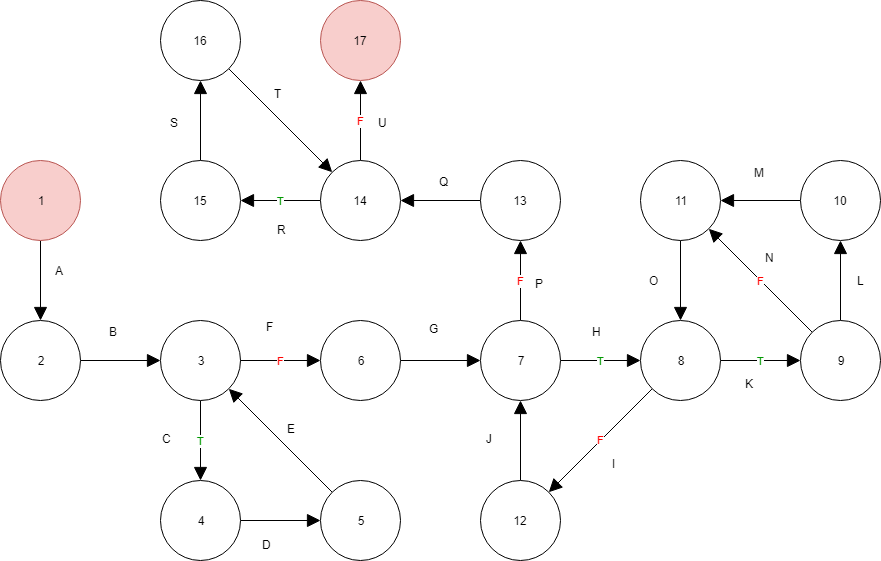
\includegraphics[width=1\textwidth,angle=0]{Struktureret_System_Udvikling/Workshop_3/Booble_Sort_Flowgraph.png}
            \caption{BubbleSort FlowGraph Diagram}
            \label{fig:BoobleSortGraph}
            \end{figure}
        \end{minipage}
        \begin{minipage}{.35\textwidth}
            \quad
            \small
            \begin{tabular}{lllll}
                1 & Before sorting\\
                2 & Print Array\\
                3 & If looped through Array\\
                4 & Print number in Array\\
                5 & Add counter in loop "Print"\\
                6 & Before Sorting\\
                7 & If looped through Array or\\
                & non Switched\\
                8 & Loop through remaining\\
                & unsorted Array\\
                9 & If current sorting pos\\
                & is bigger then next\\
                10 & Switch number possitions\\
                11 & Add counter in loop\\
                & "Remaining unsorted"\\
                12 & Add counter in loop\\
                & "Array or non Switched"\\
                13 & After Sorting\\
                14 & Print Array\\
                15 & If looped through Array\\
                16 & Print number in Array\\
                17 & Add counter in loop "Print"\\
            \end{tabular}
        \end{minipage}
    \end{table}
    \noindent
    Og kan derfor, ved en program kørsel forvente en gennemgang i ruterne:\\
    \textit{A-B-\{C-D-E\}*(Array størrelse)-F-G-\{H-\{K-[N/L-M]-O\}-I-J\}-P-O-\{R-S-T\}*(Array størrelse)-U}\\
    Hvor \{ Tuborgklammer \} definere et loop af en vis størrelse, der altid skal opfylde det beskrevne mønster.\\
    Eneste afvigelse kan ses ved \textit{N} der også kan være beskrevet ved ruten \textit{L-M}.\\\\
    Efter første gennemgang kan dog konkluderes at funktionen tager følgende rute:\\
    \textit{A-B-\{C-D-E\}*4-F-G-H-K-K-K-K-......}\\
    Derved kan ses at her forekommer 2 typer af fejl:\\
    Første i loopet mellem \textit{C, D, E} der ikke fuldender den forventede længde. Denne kan løses ved kodens forloop der skal rettes fra \code{for (int i = 0; i \textless --size; i++)} til\\ \code{for (int i = 0; i \textless = size; i++)}.
    Anden fejl forekommer i loopet ved \textit{K}, hvor man ved en nærmere kode inspektion kan se at de omkringliggende loops mangler afsluttende tuborgklammer.\\
    Efter anden gennemgang kan dog stadig ses, at funktionen ikke tager forventede rute, da næste forventede rute ville være: \textit{F-G-H-K-L-M-O-K-L-M-O...}, for det definerede array \textit{10-2-5...}, og ikke den resulterende rute: \textit{F-G-H-K-N-O-K-N-O...}\\
    Denne fejl skal findes i sorterings kodens tjek for, om et element på den givende position er større end det næste element. Koden \code{if (a[j] \textless a[i+1])} skal derfor rettes til \code{if (a[j] \textgreater a[j + 1])}, da \code{j} definerer nuværende tjek og \code{i} definerer arrayets gennemgang. Efterfølgende skal dog også bemærkes at det samme definerede \code{i}, også anvendt i koden \code{hold = a[i];}, heller ikke relaterer til den forventede position, og skal derfor af samme grund rettes til \code{hold = a[j];}.\\
    Efter sidste gennemgangs rettelser, kan den sidste fejlrettelse findes i loopet defineret fra \textit{H-J}, der ved et gennemløb bliver afsluttet inden dens forventede resultat. Altså kan fejlen findes i koden \\
    \code{for (i = 0; i \textless (size \&\& switched); i++)}, hvor der bemærkes at loopets header indeholder en forkert sat parentes \code{i \textless (size \&\& switched)} skal derfor rettes til \code{(i \textless size) \&\& switched}.
\end{document}